\begin{figure} [htbp]
  \begin{subfigure}[b]{.49\textwidth}
   \centering
   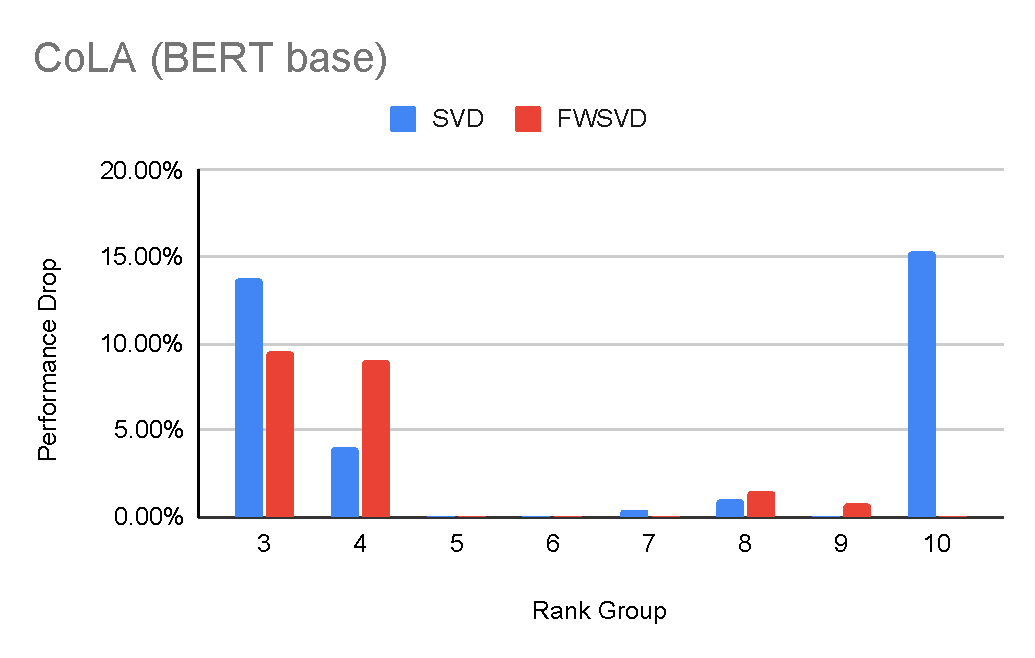
\includegraphics[width=\textwidth]{figures/group_truncation/CoLA_BERT_base.pdf}
       \caption{}
       \label{fig:rank_group_cola_bert}
       \end{subfigure}
\begin{subfigure}[b]{.49\textwidth}
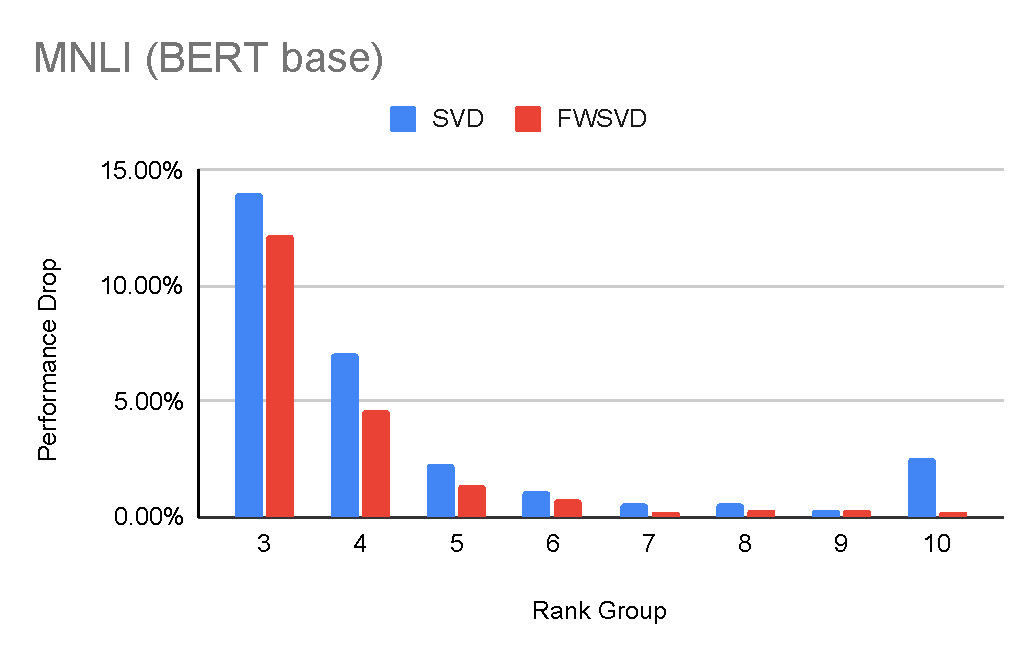
\includegraphics[width=\textwidth]{figures/group_truncation/MNLI_BERT_base.pdf}
\centering
  \caption{}
   \label{fig:rank_group_mnli_bert}
\end{subfigure}
\begin{subfigure}[b]{.49\textwidth}
   \centering
   \includegraphics[width=\textwidth]{figures/group_truncation/QNLI_bert_base.pdf}
       \caption{}
       \label{fig:rank_group_qnli_bert}
\end{subfigure}
\begin{subfigure}[b]{.49\textwidth}
\includegraphics[width=\textwidth]{figures/group_truncation/STS-B_bert_base.pdf}
\centering
  \caption{}
   \label{fig:rank_group_stsb_bert}
\end{subfigure}
\begin{subfigure}[b]{.49\textwidth}
   \centering
   \includegraphics[width=\textwidth]{figures/group_truncation/MRPC_bert_base.pdf}
       \caption{}
       \label{fig:rank_group_mrpc_bert}
       \end{subfigure}
\begin{subfigure}[b]{.49\textwidth}
\includegraphics[width=\textwidth]{figures/group_truncation/NER-CoNLL2003_bert_base.pdf}
\centering
  \caption{}
   \label{fig:rank_group_ner_bert}
\end{subfigure}
\begin{subfigure}[b]{.49\textwidth}
\includegraphics[width=\textwidth]{figures/group_truncation/QQP_bert_base.pdf}
\centering
  \caption{}
   \label{fig:rank_group_qqp_bert}
\end{subfigure}
\begin{subfigure}[b]{.49\textwidth}
\includegraphics[width=\textwidth]{figures/group_truncation/SST-2_bert_base.pdf}
\centering
  \caption{}
   \label{fig:rank_group_sst2_bert}
\end{subfigure}
\caption{This figure shows only groups 3 to 10 of Figure \ref{fig:truncation_bert} to better visualize the groups of a smaller performance drop.
}
\label{app:err_per}
\end{figure}